\chapter{Results}

This chapter is dedicated to the results obtained in experiments and the model. We start by describing the raw experimental results to get a big picture of the system. Afterward, we analyze intensity as an indirect measurement of the mean density accumulation, proving there is a transition in the accumulation near walls. Results of tracking explain further these observations.  

\section{Observations}
\label{section: observations}

In the introduction in Chapter 1, we discussed multiple effects of surfaces on bacteria. These effects appear depending on the swimming properties, body and flagella shape, and surface properties. In our experiments, we observe cell adhesion to the frontal wall when not using BSA, circular trajectories, non-zero contact angles with the flat walls causing trapping of bacteria in that wall, wall-cell alignment, and cell-cell interactions causing clustering.

\subsection{Cell adhesion}


We observe that cell adhesion to the frontal wall occurs when the surfaces are not coated with BSA. In figure \ref{adhesion} we show four frames of an experiment where BSA was not utilized. Four bacteria have adhered to the front wall. Adhesion gives rise to the biofilm formation that we want to avoid. In this case, the adhesion is of electrostatic origin and is therefore prevented by using BSA. It could be argued that using BSA affects the curved wall results in preventing adhesion and therefore should not be used. Nevertheless, we measure surface effects prior to adhesion to design a surface that allows bacteria to leave the wall. Once adhesion has occurred, bacteria will form biofilm independently of the shape of the surface. Therefore, this adhesion is not relevant to our measurements. In other terms, we are not studying cell adhesion mechanisms, so there are no reasons to measure this phenomenon. If we were measuring cell adhesion, to test our results, we should use wild-type strains where more adhesion mechanisms are present \cite{Costerton1987BacterialDisease.}. 

\begin{figure}
	\centering
	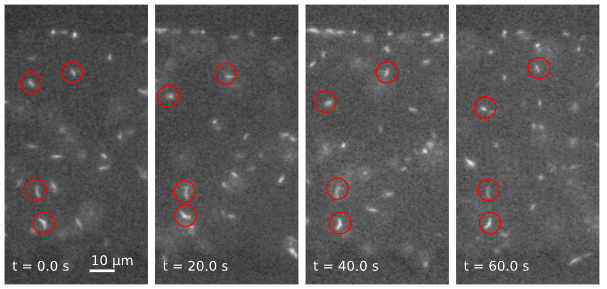
\includegraphics[width=\linewidth]{imagenes/adhesion.PNG}
	\caption[Frames of an experiment not used because the channel was not coated with BSA]{Four frames of an experiment where the channel was not coated with BSA. The four cells enclosed by red circles appear on all frames because they have adhered to the frontal surface. Adhered bacteria slightly move but never leave the focal plane. No measurements were made on these experiments. We only used them in this figure to show what happens when not using BSA. } 
	\label{adhesion}
\end{figure}


\subsection{Circular trajectories}

\begin{wrapfigure}{r}{0.5\linewidth}
\vspace{-50pt}
\centering
\includesvg[width=\linewidth]{imagenes/circular_trajectories}
\caption[Circular trajectories near walls]{Example of three circular trajectories observed in an experiment. The star indicates the beginning of a track while the triangle marks the end. The video used for this figure had 12 trajectories with circular sections of a total of 302, which correspond to $4\%$. The three shown trajectories are the longest ones.}
\vspace{-50pt}
\label{circular trajectories}
\end{wrapfigure}

We see circular swimming trajectories on the frontal surface, caused by hydrodynamic interactions between the cell and the boundary \cite{Lauga2006SwimmingBoundaries}. In figure \ref{circular trajectories} we display three example trajectories. The percentage of trajectories observed that display circular movement is $4\%$ for the experiment used for the figure. Thus, the phenomenon is marginal and, therefore, not implemented in the model. 

\label{section:cell trapping}
\subsection{Flat wall trapping}

Due to the hydrodynamic interactions when bacteria swim in contact with a flat wall, the angle of contact is not zero \cite{Sipos2015HydrodynamicWalls} as can be seen in figure \ref{trains}. This causes bacteria to swim along the surface in average for \SI{60}{\second} \cite{Drescher2011FluidScattering}. In our experiments, we observe this behavior in the two flat walls of the system, the upper and the frontal wall. Due to this effect, bacteria barely leave the focal plane, validating the two-dimensional aspect of the model. This effect has another interesting consequence. When swimming in contact with the wall, cells may encounter another cell swimming in the opposite direction, forming a pair of stagnant cells. Other cells that reach this pair will also become stagnant. After a time, typically in the order of 10 seconds, the cells manage to separate, and the bacteria that swim in the same direction leave together. This forms ``trains" of cells moving in the same direction as shown in the figure \ref{trains}. Usually, the observed trains have less than ten cells, and not all cells on the flat wall move in trains. 

 
\begin{wrapfigure}{r}{0.5\linewidth}
\centering
\includesvg[width=\linewidth]{imagenes/tren}
\caption[Observation of a train of bacteria swimming in the same direction]{Observation of a train of bacteria moving to the right in three different frames with their respective times $t$. We also see how the bacteria swim at a non-zero angle when in contact with the flat wall. The red line is the border of the ROI, representing the flat wall.}
\vspace{-50pt}
\label{trains}
\end{wrapfigure}

When a cell swimming in the opposite direction of a train collides with it, it moves into the focal plane or away from the upper wall. This occurs because the train has more mass and pushes harder than the individual bacterium displacing it. This effect causes bacteria to leave the flat wall. However, it is also possible that the bacteria do not interact with the train, as the system is three-dimensional.


\afterpage{
\begin{figure}[H]
	\centering
	\includesvg[width=\linewidth]{imagenes/trapping_merge}
	\caption[Trajectories of bacteria following the profile of the curved wall in experiments and simulation]{Four sequences of frames showing an individual bacteria going along the curve of a wall for $\lambda=$ \SI{30}{\micro\meter} and two different values of $A$, in experiments a,b) and simulations c,d). Each frame has the time $t$ on the bottom. The reference time $t=$ \SI{0}{\second} is exactly when the bacteria reach the wall. a) In this case, the amplitude is not too high, and therefore the bacterium can cross the valley in only \SI{1.5}{\second}. In the last frame, two bacteria appear, but it is clear which bacteria correspond to the previous frames if we consider the logical trajectory. b) For a higher amplitude, we observe that the bacterium stays in the same position for many seconds until it leaves. c, d) Results of simulations for  $K=$ \SI[per-mode = symbol]{3.0}{\radian \per \second}, $D_r= $ \SI[per-mode = symbol]{0.015}{\radian \per \square\second}. The arrow is the vector $\textbf{p}$. Trajectories and residence times in the simulations are similar to the experiments. The red line is the border of the ROI, representing the curved wall. }
	\label{esteric allignment}
\end{figure}
}

\subsection{Steric alignment with the wall}

When bacteria hit the wall, they experience a torque that aligns them with the wall, as described in section \ref{section:steric alignment}. For the flat wall, this effect means that after about 1 second, the bacteria are aligned with the wall. Aligned means that the bacterium swims with a stable non-zero angle, as mentioned in section \ref{section:cell trapping}. On the other hand, the effect is much more interesting for the curved wall and it depends on the values of the amplitude $A$ and the wavelength $\lambda$. We remember that $A$ and $\lambda$ have units of \SI{}{\micro\meter}. In figures the units will be omitted for simplicity. The torque allows the bacteria to follow the profile of the wall. Hydrodynamic interactions can cause bacteria to follow convex walls such as peaks \cite{Sipos2015HydrodynamicWalls}, but for the curvatures we are working with, this is rarely observed. Therefore, once they reach a peak, they stop feeling the steric torque and leave the wall. Only for $A=$ \SI{2.9}{\micro\meter} and $\lambda=$ \SI{30}{\micro\meter} some bacteria follow the sinusoidal shape of the wall. However, for high values of $A$ and low wavelength $\lambda$, bacteria could be trapped in the valley for a considerable time. This entrapment of cells in the curved wall can be due to a couple of reasons. In the case where there is only a single point of contact, we can understand this phenomenon by looking at the equation \eqref{eq:wall alignment}. For curved walls with high curvature, the vectors $\hat{\textbf{t}}_w$ and $\hat{\textbf{n}}_w$ vary significantly in space. This implies that as the bacteria swims parallel to the valley, the value of the dot product $\hat{\textbf{n}}_w \cdot \textbf{p}$ will stay close to zero even if the bacteria rotates. This causes the bacteria to rotate slowly and stay in the valley for longer times. Also, in the most extreme cases, corresponding to high $A$ and low $\lambda$, the bacteria may have several contact points with the wall, both with the body and the flagella, resulting in the bacteria being unable to rotate at all. 

In the figure \ref{esteric allignment} a, b) we show two individual cells whose trajectories illustrate the previously described phenomena. In sequence a) the amplitude is small enough for bacteria to move along the valley in \SI{1.5}{\second}. This is precisely what we are looking for. If bacteria can follow the wall curve and leave it in an interval of time lower than the characteristic adhesion time, we could reduce biofilm formation. In contrast, sequence b) shows how a bacterium spends too much time in the valley due to the reasons previously discussed. This will undoubtedly lead to adhesion in an in vivo environment. In the following sections \ref{section:intensity} and \ref{section: tracking} we will further investigate the behavior of bacteria on these surfaces by measuring the average density and speed when in contact with the wall. 

In simulations we observe a similar behavior. In figure \ref{esteric allignment} c, d) we show trajectories of particles with the parameters $K^*=$ \SI[per-mode = symbol]{3.0}{\radian \per \second} and $D_r^*= $ \SI[per-mode = symbol]{0.015}{\radian \per \square\second}. In section \ref{section:intensity} we will compare different values of $K$ and $D_r$ and it will be clear why these values were chosen for this figure. For now, we can observe that the model replicates the behavior in the valley, and also quantitatively the times are in the same order of magnitude. 


\label{section: clustering} 
\subsection{Clustering}

The phenomenon of bacteria trapping in the curved wall observed in figure \ref{esteric allignment} b) can be significantly increased when bacteria collide in the valley. For multiple bacteria colliding in one valley it is impossible for them to reorient and leave the wall. This will increase adhesion and the formation of biofilm. In figure \ref{clustering} we show two clusters of bacteria in a valley that were formed in the most extreme cases of amplitudes. The valley is very narrow, so bacteria stay in it for around \SI{10}{\second} even if alone. When other bacteria reach the valley, their movement is further restricted, and they cannot leave the wall. These clusters will last for several seconds, in some cases even for the entire video duration. We show representative examples where the clusters grow but also, sometimes, the cluster lose bacteria and even dissolve. Nevertheless, in a more natural environment, bacteria will adhere and then divide, and therefore biofilm will form. 

It is important to mention that this situation also occurs in walls with smaller amplitude, only less frequently. In figure \ref{cluster with low amplitude}, we show a case where this occurred for $A=$ \SI{2.9}{\micro\meter} and $\lambda=$ \SI{27}{\micro\meter}. Two bacteria collide and start a cluster, but shortly after, the cluster is dissolved when at time $t= $ \SI{13}{\second} two cells approach the cluster. These cells push the cluster causing all bacteria to align and leave the surface, as seen in  $t= $ \SI{14}{\second}. Cell-cell interactions play an important role in the dynamics of the system. We observe that cell-cell alignments can cause bacteria to leave or become trapped on the surface. The main difference between the cases of figures \ref{clustering} and \ref{cluster with low amplitude} is the effect that the cell-wall interaction produces. Cell-wall interactions could trap bacteria for several seconds if the valley is too narrow. Other bacteria will reach the valley, and a cluster will form, leading to residence times around \SI{100}{\second}. On the contrary, if cell-wall alignment contributes to bacteria leaving the wall quickly, cell-cell interactions are more infrequent and interrupt bacteria for less time, and therefore the accumulation in the surface will be reduced. The contribution of the steric alignment with the wall is the key to controlling accumulation on the surface.

\begin{figure}[H]
	\centering
	\includesvg[width=\linewidth]{imagenes/clustering}
	\caption[Clusters formed in valleys of the most ]{Clusters of bacteria formed in narrow valleys. Multiple bacteria collide and interrupt their movement, causing extremely long residence times. In both cases, $t=0$ corresponds to when the cluster was formed. a) The cluster was formed when two bacteria arrived almost simultaneously at a valley already occupied by a trapped cell. The cluster does not dissolve as the video ends in $t\sim$ \SI{130}{\second} and two bacteria remain in the valley. b) Another example where the cluster lasted for more than \SI{100}{\second} until it dissolved. The red line is the border of the ROI, representing the curved wall.}
	\label{clustering}
\end{figure}

\begin{figure}[H]
	\centering
	\includesvg[width=\linewidth]{imagenes/collison_low_A}
	\caption[Collision in a curved wall with low amplitude]{Example of a collision in a curved wall with a low amplitude. The residence time of bacteria involved in the collision is about \SI{10}{\second} while in figure \ref{esteric allignment} a) we observe a residence time of \SI{1.5}{\second} for a even more curved wall. The red line is the border of the ROI, representing the curved wall. }
	\label{cluster with low amplitude}
\end{figure}

\afterpage{
\begin{figure}[H]
	\centering
	\includesvg[width=\linewidth]{imagenes/clustering_simulation}
	\caption[Comparison in simulations between values of $k_{\text{cell}}$ in the high curvature case]{Comparison in simulations between values of $k_{\text{cell}}$ in the high curvature case. a) case with $k_{\text{cell}}=0$. In $t=$ \SI{0}{\second} three particles reach the valley, at $t=$ \SI{46}{\second}, more particles arrived on earlier frames but also particles start leaving the valley, independently of each other. The valley is empty at $t=$ \SI{65}{\second}. b) case with elastic interactions $k_{\text{cell}}=$ \SI{500}{\per\second}. In  $t=$ \SI{0}{\second} an initial bacterium occupies a valley and at $t=$ \SI{16.5}{\second} a second bacterium arrives. The collision between these two cells fixes the value of the the vector $\hat{\textbf{t}}_w$ to which bacteria align, allowing bacteria to leave only \SI{4}{\second} after the collision. }
	\label{clustering simulation}
\end{figure}}

\newpage

On the other hand, we consider an elastic interaction between the cells in the simulations. This interaction makes sense for spherical particles; however, it is not enough to capture what happens when clusters form in the valleys of the curved wall. The alignment between cells is relevant to describe cluster formation. When several bacteria collide in a valley, they disrupt each other and cannot follow the curve of the wall. In the figure \ref{clustering simulation} we show two simulation results for $A=$ \SI{10}{\micro\meter}, $\lambda=$ \SI{21}{\micro\meter} for two values of the elastic cell interaction $k_{\text{cell}}=$ \SIlist[list-units=single]{0;500}{\per\second}. In the case without interactions, bacteria reach the valley and share a similar position. The trapping time is large and around \SI{50}{\second}. The moment bacteria leave the cluster is completely independent of the other cells. Therefore, this is not a cluster of bacteria, but rather individual bacteria trapped for long times. The problem is that when we consider an interaction between cells, a meaningless dynamic appears. If two bacteria meet in the valley, the elastic force immobilizes both bacteria, which means that the vectors $\hat{\textbf{t}}_w$ and $\hat{\textbf{n}}_w$ remain constant for each bacterium. In a short time interval, both cells align with the vector $\hat{\textbf{t}}_w$ so they can leave the wall. The situation were $\textbf{p}\cdot\hat{\textbf{n}}_w \approx 0$ is broken by the collision of bacteria. 

We conclude that the model will underestimate the accumulation in the valley for cases with high curvature because it does not predict cluster formation. The best scenario for the model is to consider $k_{\text{cell}}=0$, so bacteria only accumulate due to the correctly modeled trapping in the valley. Since we are working on a low-density regime in experiments, we think that this simplification is plausible. This means that the optimal values of the model may not be applicable for high-density regimes where clustering forms more frequently. A more complicated model should consider cell-cell alignment to reproduce the clustering phenomena in the valley correctly. We will try to implement those interactions before publishing this work.
 
\label{section:intensity}
\section{Mean intensity}

The methodology described in section \ref{section: noise remove} allows us to consider the signal measured as coming solely from the fluorescence of the bacteria. Therefore the mean intensity registered in the experiments is an indirect measurement of bacteria density. We will measure mean intensity over a period. We begin by showing examples of the two-dimensional mean intensity and the effects of the previous observations in this quantity. Afterward, we describe intensity profiles $I(x)$ for the curved wall. These profiles exhibit a transition in their behavior that corresponds to what was observed in the section \ref{section: observations}. This will allow us to quantify the qualitative behavior exhibited by the system due to the alignment with the wall. 

\afterpage{
\begin{figure}[H]
	\centering
	\includesvg[width=\linewidth]{imagenes/2d_density}
	\caption[Mean intensity over a period for different values of $A$ and $\lambda$]{Mean intensity over a period $D_{xj}$ for different values of $A$ and $\lambda$. We choose the extreme values $\lambda =$ \SIlist[list-units=single]{21;30}{\micro\meter}. The brightness and contrast of the color scale was adjusted to improve the image display.  }
	\label{2d density}
\end{figure}
}

\subsection{Two-dimensional mean intensity}

We begin by showing results for $D_{xj}$ as defined in equation \eqref{eq:2d density}. $D_{xj}$ is the mean intensity over a period. In figure \ref{2d density} we show mean intensities over a period of the curved wall, for experiments with $\lambda =$ \SIlist[list-units=single]{21;30}{\micro\meter} and three different amplitudes. First, we note that intensities are not directly comparable between experiments, either because there is a different number of bacteria or because the bacteria fluoresce less intensely due to prolonged exposure. It is important to compare considering this aspect.

Nevertheless, it is clear that bacteria accumulate on the flat wall in all cases, but on the curved wall, the behavior depends on $A$ and $\lambda$. For low values of $A\approx$ \SI{3}{\micro\meter}, the curved surface presents fewer bacteria than the flat surface, as bacteria leave the wall when they reach a peak. As we increase the amplitude, we see how bacteria become trapped in the valley and eventually form clusters with high intensity. We call this transition the accumulation transition. The value of $A$ at which the bacteria become trapped depends on the wavelength $\lambda$ as can be seen when comparing experiments with similar amplitude \ref{2d density} b) and d). For all $\lambda$ we can observe the accumulation transition, meaning that at least there is an amplitude in which bacteria are trapped and another in which they are not.

These graphs also allow us to observe how the bacteria behave once they come out of the wall. In graphs b), e), and in particular f), it is possible to observe a darker zone near the valley. This is because once the bacteria leave the valley, they are unlikely to pass through this zone, as the angle at which they leave the wall is high. In the low amplitude case, a) and d), the amplitude is such that the bacteria stay close to the wall zone, and therefore this zone of depletion is not observed. Finally, in figure c) we observe that the curved wall only presents a high intensity on the valley. This means that clustering occurs, and so bacteria barely leave the valley, corresponding to the dynamics observed in \ref{section: clustering}. 

We observe that the average intensity captures various effects caused by the dynamics of the system. Accumulation on the flat wall, valley stagnation, and cluster formation. This reaffirms the usefulness of analyzing the average intensity to understand the system. The fact that the average intensity manages to capture the dynamics of the system should not be a surprise, as this is an indirect measure of bacteria density. 





\afterpage{%
\begin{figure}[H]
	\centering
	\includesvg[width=\linewidth]{imagenes/experimental_profiles}
	\caption[Experimental intensity profiles]{Experimental normalized intensity profiles $I(x)$ for a) $\lambda= $\SI{30}{\micro\meter} and b) $\lambda=$ \SI{24}{\micro\meter} with three different amplitudes. The colors were chosen so that curves associated with similar values of $A$ share color. The amplitudes that are shown allow to see the accumulation transition. Errorbars are the confidence interval of $95\%$ for the estimation of the mean $I(x)$. }
	\label{experimental profiles}
\end{figure}
}

\subsection{Intensity profiles}

The mean intensity matrix $D_{xj}$ has enough information to describe the system. Nevertheless, it also has two problems. It is not easy to compare due to differences in intensities between experiments, and it contains information of the bulk in the system that is not relevant for the measure of accumulation in the surface. Therefore, we consider the normalized mean intensity profiles $I(x)$ defined by equations \eqref{eq:Intensity profile} and \eqref{eq:Intensity profiles in simulations} for experiments and simulations respectively. These profiles are an average of the intensity in a zone \SI{4}{\micro\meter} normalized by the mean intensity in a \SI{4}{\micro\meter} thick zone from the flat wall. Thus, $I(x)$ indirectly measures the mean bacteria density in contact with the curved wall as compared to the flat wall. Experiments performed on different days do not show exactly the same profiles, as motility and density vary slightly, but thanks to this normalization, they are comparable. Therefore the average profile can be taken over all the experiments with the same curved wall parameters $A$, $\lambda$.   

In figure \ref{experimental profiles}, we show examples of experimental intensity profiles for $\lambda=$ \SI{30}{\micro\meter} and $\lambda= $ \SI{24}{\micro\meter} for three different amplitudes $A$. For low values $A$, the wall is slightly curved, and bacteria can move along it easily. The curvature makes bacteria leave the wall, therefore, the normalized intensity values are lower than 1. Also, there is a minimum at $x=0$ corresponding to the valley of the curved wall. This minimum is produced because not all cells touching the wall will go through the valley. If the contact starts near a peak, the cell will leave the wall without going through the whole period. Then, we have a critical amplitude, where $I(x)$ looks flat, which can be seen for $A=$ \SI{8.5}{\micro\meter} and $\lambda= $ \SI{30}{\micro\meter}. In this case, bacteria are still moving quickly around the wall, as the intensity is lower than the flat wall. Moreover, the intensity is lower than the previous case because bacteria leave the wall at a greater angle with respect to the wall axis. Finally, if the valley is too narrow, the intensity will greatly increase as bacteria get trapped. The more narrow the valley is, the higher the intensity peak as bacteria get trapped for longer times.

We can see how the profiles depend on both $A$ and $\lambda$ and conclude that $I(x)$ captures the accumulation transition successfully. This is relevant because we are considering less amount of data, but we are still representing the system correctly. We now present a quantitative description of the accumulation transition via the intensity profiles.

\subsection{The $c_1$ coefficient}

Qualitatively, the accumulation transition can be described as going from fewer bacteria in the valley of the wall to bacteria accumulating in there. This is represented by going from a minimum to a maximum at $x=0$. To quantify that aspect, we used the Fourier coefficient $c_1$ of the mean normalized intensity profile $I(x)$, calculated as:

\begin{equation}
    c_1 = \frac{2}{\lambda}\int_{-\lambda/2}^{\lambda/2} I(x)\cos\left(\frac{2\pi x}{\lambda} \right)dx = \frac{2}{\lambda} \sum_i I(x_i) \cos\left(\frac{2\pi x_i}{\lambda} \right)\Delta x,
\end{equation}

where $\Delta x=$ \SI{0.32}{\micro\meter} is the spatial resolution of the profiles and $x_i$ is the $i$-th position in the profile. Negative values of $c_1$ indicate a minimum on $x=0$ and positive $c_1$ the opposite.

\afterpage{%
\begin{figure}[H]
	\centering
	\includesvg[width=\linewidth]{imagenes/c1}
	\caption[Coefficient $c_1$ for experiments and simulations]{Color plots of the $c_1$ coefficient in the $A$, $\lambda$ parameter space. The colors are such that $c_1=0$ corresponds to the gray color and extreme negative and positive values are blue and red, respectively. a) Experimental results for $c_1$, where the number above each point represents the total number $N$ of periods considered in the average of equation \eqref{eq:Intensity profile}. b)--f) plots correspond to results from numerical simulations with their respective parameters indicated on the label. See text for more details. }
	\label{c1 coefficient}
\end{figure}
\newpage
}

Figure \ref{c1 coefficient} shows color plots of experiments and simulations for $c_1$ in the  ($\lambda$, $A$) parameter space, with red points representing an accumulation of bacteria in the valleys of the wall and blue points representing depletion of bacteria from the valleys. The transition from negative to positive values is seen in gray. The dashed line represents a two-dimensional interpolation of the curve where $c_1=0$, using an adapted version of the marching squares algorithm for irregular grids. We call the curve where $c_1=0$ the critical curve. In experiments, we can see how the accumulation transition occurs near $A= $ \SI{8.5}{\micro\meter}, $\lambda=$ \SI{30}{\micro\meter} and $A=$ \SI{5.6}{\micro\meter}, $\lambda= $ \SI{27}{\micro\meter}, but for the other wavelengths we lack the resolution in the amplitude to observe the critical amplitude $A$. We only know that it happens between $A=$ \SI{3}{\micro\meter} and \SI{5}{\micro\meter} as the dashed line indicates. 

In simulations, we show results for five different pairs of parameters $K$, $D_r$.  We remember that units of $D_r$ and $K$ are \SI[per-mode = symbol]{}{\square\radian\per\second} and \SI[per-mode = symbol]{}{\radian\per\second}, respectively. Units will not explicitly accompany values of the parameters for simplicity. In figure \ref{c1 coefficient} b) the pair of parameters $K^*=3.0$ and $D_r^*=0.015$ is the best fit for the values of $c_1$. We calculated the best fit as the set of parameters with the least square error compared to the experiments, without considering the experiments with $A\approx$ \SI{9}{\micro\meter}. We excluded those experiments because they have the least amount of realizations and show strange values of $c_1$ specially for $A= $ \SI{7.9}{\micro\meter}, $\lambda=$ \SI{21}{\micro\meter}. We only have experiments performed on a single day for those values of $A$. Unfortunately, our camera suffered a technical problem that produces condensation due to air infiltration into the sensor chamber. The camera is not available for new experiments in the mid-term. If these experiments are considered in the fit, the optimal pair only changes $D_r$ to $D_r^*=0.01$, but the fit is clearly worse.

Figures \ref{c1 coefficient} c) to f) demonstrate that not all pairs of parameters $K$, $D_r$ represent the accumulation transition trivially and also provide a notion of what results when varying the parameters. In c) and d) we use the same value of $D_r^* =0.015$ and change $K$. The case c) where $K=1.5$ predicts the critical curve for lower amplitudes than b), while d) the opposite. The interpretation is direct because $K$ controls the intensity of the alignment. Higher $K$ means bacteria move more easily along the valley and therefore are trapped less time, meaning the critical curve occurs at higher curvature. In contrast, figures e) and f) show what happens when $K^*=3.0$ is fixed and $D_r$ changes. When we increase the value of $D_r$ the transition occurs for lower amplitudes. This is because a higher thermal noise interrupts the alignment process. Nevertheless, when comparing the values of $c_1$ in $A= $ \SI{10}{\micro\meter}, $\lambda=$ \SI{21}{\micro\meter} we observe that increasing $D_r$ reduces that value. When cell trapping in the valley occurs, the steric torque is almost zero because bacteria are nearly perpendicular to the surface for a long time. Therefore, thermal noise can contribute to rotating bacteria more and reduce the residence time. Depending on the values of $A$ and $\lambda$, the coefficient $D_r$ may or may not contribute to the alignment to the wall.  



\begin{wrapfigure}{r}{0.5\linewidth}
% \vspace{-50pt}
\centering
\includesvg[width=\linewidth]{imagenes/c1_candidates}
\caption[Comparison of the accumulation transition curves for different values of $K$ and $D_r$]{Critical curves for different candidates compared to the experimental critical curve. The $c_1$ values correspond to the experimental values. We observe a parabolic shape for the critical curve. }
% \vspace{-50pt}
\label{c1_candidates}
\end{wrapfigure}


We conclude that $K$ and $D_r$ have opposite effects for the accumulation transition. Higher values of $K$ mean that bacteria align with the wall more quickly, but higher $D_r$ introduces more thermal noise that can make bacteria rotate bacteria against the wall alignment. Considering this opposite effect, many combinations of $K$ and $D_r$ can replicate the critical curve. We will call candidates, such pairs of $K$ and $D_r$ that replicate the critical curve similar to \ref{c1 coefficient} b). In figure \ref{c1_candidates} we show the critical curves for four candidates, compared to the experiment. None of the candidates exactly replicate the critical curve, specially due to the value $c_1=0.02$ for $A=$ \SI{8.5}{\micro\meter} and $\lambda= $ \SI{30}{\micro\meter} in experiments.

To understand this better, figure \ref{candidates intensity profiles} shows intensity profiles obtained in simulations of candidates, compared to the measured in experiments for values of $A$ and $\lambda$ that are of interest for the transition. The experiment's intensity profiles are subject to various effects that the simulations do not capture. For example, some experimental profiles are asymmetric due to inhomogeneities in density, causing more bacteria to come from one side, as observed in g), h), and i). However, this is not the only significant difference. In profiles d), e), and f), we see that the simulations do not predict a drop in the intensity values when the accumulation transition occurs; only the shape of the profile is adequately predicted, especially by the $K^*=3.5$, $D_r^*=0.015$ case. The experimental intensity profiles reach near-zero negative values for these cases, probably because we overestimated the mean noise for these cases. Also, in c), the experimental profile is flat, so $K=5.0$ is the closest curve, differing from the previous case.

\afterpage{
\begin{figure}[H]
	\centering
	\includesvg[width=\linewidth]{imagenes/candidate_profiles}
	\caption[Comparison of intensity profiles within experiments and four simulation candidates]{ Normalized intensity profiles for experiments and four simulation candidates. Rows have similar amplitude $A$, and columns have the same wavelength $\lambda$. The horizontal and vertical scales are adjusted depending on the amplitude and wavelength to pursue a clear display of the data. We only show representative candidates as many values represent the transition. Experimental error bars are the $95\%$ confidence interval for estimating the mean normalized intensity $I(x)$. The complete set of normalized intensity profiles is in appendix A. }
	\label{candidates intensity profiles}
\end{figure}
\newpage

\begin{figure}[H]
	\centering
	\includesvg[width=\linewidth]{imagenes/c1_curvature2}
	\caption[Coefficient $c_1$ as function of the curvature $\kappa$]{ Comparison between $c_1$ values for experiments and simulations with the best set of parameters. The dots enclosed by red circles correspond to $A\approx$ \SI{9}{\micro\meter} and were not considered for the fit. The inset is a close up to the low values of $\kappa$. The dashed line of the inset corresponds to $c_1=0$}
	\label{c1 curvature}
\end{figure}
}

We conclude that there is no perfect candidate to replicate the exact results of all experiments. A possible solution is to redefine the parameter of $K$ as a function of $A$ and $\lambda$. However, how exactly will $K$ depend on these parameters and what is the rationale behind that are important questions. A model with more parameters can fit anything, not necessarily meaning that the model is better. The simpler version of the model is close in behavior for all candidates compared to the experiments. We believe that cell-cell alignment is the only missing aspect of the dynamics and that may be enough. 

The $c_1$ coefficient quantifies the qualitative behavior observed in $I(x)$ with only one scalar, so it is an oversimplication. Color plots of $c_1$ in the $(\lambda, \ A)$ parameter space reveal information about where the transition occurs. The fact that candidates of parameters replicate the plot should be interpreted as a qualitative replication of the results in the experiments. Exact quantitative predictions for all the profiles are not achievable with this model with only two parameters $K$, $D_r$. Due to this, we decided to show many candidates instead of just the overall better fit.

Finally, we observe an important aspect of $c_1$. All critical curves resemble a parabolic shape, presuming that there would be a relation between $A$ and $\lambda^2$ that defines the critical curve. This is not a coincidence because the maximum curvature in the sinusoidal wall is given by $\kappa=4\pi^2A/\lambda^2$. The shape of the critical curves indicates that there is a relation between the curvature $\kappa$ and $c_1$. To visualize this in figure \ref{c1 curvature} we show $c_1$ as a function of $\kappa$ for the experiment and the simulation using the best fit $K^*$ and $D_r^*$. As mentioned previously, we neglect the measures for the experiments with $A\approx$ \SI{9}{\micro\meter}. Without considering these data, the model quantitatively replicates the measurements. The quantitative agreement indicates that the model effectively captures the accumulation transition when it is parameterized by $c_1$.  

\newpage

\begin{wrapfigure}{r}{0.5\linewidth}
% \vspace{-50pt}
\centering
\includesvg[width=\linewidth]{imagenes/c1_curve_with_curvature}
\caption[Comparison of the accumulation transition curves for experiments and the optimal set of parameter with the curvature define by constant curvature $\kappa^*=0.3$]{Comparison of the accumulation transition curves for experiments and the optimal set of parameter with the curvature define by constant curvature $\kappa^*=0.3$. The $c_1$ values correspond to the experimental values.  }
\label{c1 curvature fit}
\end{wrapfigure}

Looking at the inset of figure \ref{c1 curvature}, the critical curvature at which $c_1=0$ is around $\kappa^* =$ \SI{0.3}{\per \micro \meter} as the experiments with $A=$ \SI{5.6}{\micro\meter} and $\lambda=$ \SI{27}{\micro\meter} indicates. In figure \ref{c1 curvature fit} we show a comparison of the critical curves of the experiment and the optimal pair of parameters, compared to the curve defined by fixing the curvature $\kappa^* =$ \SI{0.3}{\per \micro \meter}. More resolution on the values of $A$ and $\lambda$ will allow to determine the position of the critical curve and the corresponding critical curvature better. 


The dependence with respect to $\kappa$ is really important because it defines a surface parameter for the accumulation transition independent of the sinusoidal shape of the curved surface. Other surface designs with their own properties may be adapted to have an optimal curvature that allows a geometric control of the accumulation. For example, in the Sharklet design \cite{Reddy2011MicropatternedColi} a semicircle connection between the microscopic structures of the appropriate radius will reduce the accumulation of cells in the surface. Compared with the natural forms observed in sharkskin, where there is a curvature, this idea is promising.


\afterpage{%
\begin{figure}[H]
	\centering
	\includesvg[width=\linewidth]{imagenes/mean_intensity_6comparison}
	\caption[Mean intensity in the $A$, $\lambda$ parameter space for experiments and simulations]{Mean intensity $\langle I(x) \rangle$ as function of $A$ and $\lambda$. We used the gray color for $\langle I(x) \rangle=1$, meaning there is the same accumulation in the flat and curved wall. Therefore, blue dots mean the curved wall contributes to less accumulation, and red the opposite. a) In experimental results, there is a decrease in the accumulation not predicted in the simulations. This reduction corresponds to where the accumulation transition occurs. b)--f) plots correspond to results from numerical simulations with their respective parameters indicated on the label.}
	\label{mean intensity}
\end{figure}
\newpage
\begin{figure}[H]
	\centering
	\includesvg[width=\linewidth]{imagenes/meanI_curvature}
	\caption[Mean normalized intensity $\langle I(x) \rangle$ as function of the curvature $\kappa$]{ Comparison of $\langle I(x) \rangle$ between experiments and simulations with the best set of parameters. We observe a minimum in the mean of the normalized intensity for experiments but such behavior is not captured by the model. The red circles enclose experiments with $A\approx$ \SI{9}{\micro\meter}}
	\label{meanI curvature}.
\end{figure}

}

\subsection{Mean of the normalized intensity}

While $c_1$ characterizes when the accumulation transition takes place, it does not directly measure the total accumulation of bacteria. Therefore, we consider the average normalized intensity $\langle I(x) \rangle$ to quantify the total accumulation compared to the flat wall. In figure \ref{mean intensity} we show $\langle I(x) \rangle$ as function of $A$ and $\lambda$ in the same configuration as figure \ref{c1 coefficient}. For this case, we use the gray color for $\langle I(x) \rangle =1$, meaning there are an equal density of bacteria in the curved and flat wall. The orange dashed line corresponds to the interpolation of the curve where $\langle I(x) \rangle =1$, while the black one is the critical curve of the accumulation transition. In a) the experimental results show how the average intensity follows a similar pattern as the coefficient $c_1$ seen in figure \ref{c1 coefficient}. As the curvature of the wall increases, so does the average intensity, obviously due to the trapping of bacteria. Nevertheless, there is a minimum of $\langle I(x) \rangle$ on the values of $A$ and $\lambda$ where the accumulation transition occurs. The model fails to predict this minimum. Instead, the simulations show virtually no variation in the average intensity in the region with $c_1\approx0$. 

Figures \ref{mean intensity} c)-f) show the comparison for different parameters. This plot supports the idea previously discussed with the $c_1$ coefficient. Comparing c) with d), we also see that increasing $K$ the accumulation in the wall is reduced. In d), the value of K produces $\langle I(x) \rangle <1$ for all $A$, $\lambda$ preventing the orange curve from being seen. Meanwhile, figures e) and f) show how the accumulation is decreased for higher values of $D_r$. Two effects interplay in this situation. First, as discussed in the previous section, the effect of $D_r$ when bacteria stagnate favors the release of bacteria from the wall with high curvature. Second, a higher $D_r$ increases the rate at which particles in the flat wall turn away from it. Therefore, increasing $D_r$ reduces the accumulation of bacteria in the flat wall as well. This decreases the normalization constant, and so it increases the relative accumulation in the curved wall measured by $\langle I(x) \rangle$. Nevertheless, comparing e) and f), it appears that the first effect dominates because the accumulation decreases.

In figure \ref{meanI curvature} we show the mean normalized intensity as a function of the curvature $\kappa$. We observe that the quantitative predictions fail in the region between $\kappa = $ \SIlist[list-units=single]{0.2;0.4}{\per\micro\meter} as discussed previously. This is precisely where the accumulation transition occurs; therefore, the bacteria begin to stagnate in the valley, increasing the accumulation. The only possible explanation for the decrease in the intensity of the experiments is that for these intermediate curvatures, bacteria leave the wall at a considerable angle, increasing the probability that they will move away from the curved wall. This will be confirmed in section \ref{section: times}. Simulations do predict the reduction of the mean intensity as the values are slightly smaller at that point, but not quantitatively. We think that this difference between simulation and experiments may be due to an overestimation of the average noise in the curved wall for the experiments, caused by low-intensity bacterial pixels such as those of bacteria swimming out of focus. A more detailed calculation of the noise may be necessary. 


\label{section: tracking}
\section{Tracking}

Following the methodology described in section 2.2.4, we track bacteria movement. The method determines bacteria position $\textbf{r}_i$ for each frame and then form links between detections to create the trajectories. This is an automatic process subject to errors but mostly gives correct results. We can calculate the bacteria velocity $\dot{\textbf{r}}_i$ by using equation \eqref{eq tracking velocity}. In simulations both, $\textbf{r}_i$ and $\dot{\textbf{r}}_i$ are numerically calculated on each time step. Statistics of these vectors will reveal more information about the system's dynamics.

\afterpage{%
\begin{figure}[H]
	\centering
	\includesvg[width=\linewidth]{imagenes/speed_distribution}
		\caption[Probability density functions for the normalized speed in contact with the curved wall.]{Probability density functions for the speed in two different experimental videos for $\lambda= $ \SI{30}{\micro\meter} and $A=$ \SI{5.6}{\micro\meter}. a) and b) distributions for the non-normalized speed $V$ in the bulk and the curved wall, respectively. c) and d) distributions for the normalized speed $v=V/V_{\text{bulk}}$ in the same experiments. a) shows distributions in bulk with different means, but in c) we can see how the distributions in bulk are comparable, thus justifying the usage of the normalized speed instead of $V$.	}
	\label{speed distribution}
\end{figure}
}

\subsection{Speed distribution}

We begin by considering the probability density function (pdf) of the speed $V$. Caution is required when comparing that quantity for different experiments. Cell motility is not always the same. It is affected by the use of the micropipette, the presence of oxygen, and centrifugation. In figure \ref{speed distribution} we show normalized histograms representing the pdfs of speed for experiments with $\lambda=$ \SI{30}{\micro\meter} and $A=$ \SI{5.6}{\micro\meter} made in two different days. Figure \ref{speed distribution} a) shows the pdf for the speed in the bulk of the system, namely far from both walls. The speed distribution for day 1 is broader, and its mean is higher than on day 2. Figure \ref{speed distribution} b) shows the speed distribution in contact with the curved wall and presents the same differences. In the bulk of the system, bacteria speed distributes Gaussian-like, but when in contact with the wall, bacteria slow down due to the trapping in the valley.

To avoid differences between experiments of different days, we use the normalized speed $v=V/V_{\text{bulk}}$ to compare between different experiments, where $V_{\text{bulk}} = \langle V \rangle_{\text{bulk}}$ is the mean speed in the bulk of the system for a specific video. In figures \ref{speed distribution} c) and d) we plot the pdf of the normalized speed. This normalization ensures that experiments have comparable distributions similar to the normalization of intensity by the average of the flat wall. We will compare the normalized dimensionless speed $v$, so experimental measures can consider all experiments that share the same $A$ and $\lambda$ values. The fact that normalization works for the pdf in contact with the curved wall is not trivial. However, it is explained by the observation that the interactions with the wall are proportional to the speed of the bacteria, as shown in equation \eqref{eq:steric_force}. Therefore, if we divide by $V_{\text{bulk}}$ the mean speed of an individual bacteria when swimming free and redefine the normalized velocity $\dot{\textbf{r}}/V_{\text{bulk}}$, the dynamics are rescaled and independent of the mean speed in bulk.

\afterpage{%
\begin{figure}[H]
	\centering
	\includesvg[width=\linewidth]{imagenes/speed_distribution_comparison}
	\caption[Probability density functions for the normalized speed in contact with the curved wall]{Experimental probability density functions of speed in contact with the curved wall. We only display experimental results, as in simulations we do not consider a distribution of mean speeds for particles, and therefore, simulations are not comparable. The accumulation transition is represented by a shift of the pdf to the left and an increase in the probability of having bacteria with $v\approx0$ corresponding to stagnation in the valley.}	
	\label{speed distribution: comparison}
\end{figure}
\newpage
}

In figure \ref{speed distribution: comparison} we show experimental results for speeds in contact with the curved wall for different values of $A$ and $\lambda$. For low values of the amplitude $A$ g), h) and i) show that bacteria move almost at $v=1$, and the distribution looks like a trunked Gaussian. When the curvature increases, the distribution moves towards the $v=0$ value for the highest curvatures, a peak at $v=0$ appears, and the distribution looks like an exponential distribution. This is a direct measure of the trapping of bacteria. Comparing with figure \ref{candidates intensity profiles}, it is possible to observe that the accumulation transition corresponds to this shift of the distribution towards zero speed values and also the formation of the peak at $v=0$. We do not compare experimental results with simulations because we did not consider a distribution of speeds for particles in the model.

\subsection{Speed profiles}

Speed profiles are conceived similarly to intensity profiles. If a particle $i$ is in the band of the curved wall with position $\textbf{r}_i =(x_i, y_i)$, we can assign an interval where $x_i$ is contained in the $x$-axis as $[x-\Delta x/2,x+\Delta x/2]$ defined by its center $x$. This creates a set of observations $\mathcal{O}_x$ associated with the interval defined by $x$. For each value $x$, we define $v(x)$ the mean speed in the set of observations $\mathcal{O}_x$ that are inside the interval. Particles in the band are probably in contact with the wall, so vertical position does not reveal more information. The definition is the same for experiments and simulations, but in experiments $\Delta x $ = \SI{1}{\micro\meter} is considered, while in simulations $\Delta x $ = \SI{0.32}{\micro\meter} as usual in the intensity profiles. The reason for this change for the experiments is that in the less frequented positions, by losing resolution, it is possible to increase the size of $\mathcal{O}_x$ in those positions. This is essential for the cases where bacteria are trapped in the valley. Figure \ref{velocity profiles} h) shows a case where two points have a high errorbar due to the small size of $\mathcal{O}_x$.

\afterpage{%
\begin{figure}[H]
	\centering
	\includesvg[width=\linewidth]{imagenes/velocity_profiles}
	\caption[Speed profiles compared between experiments and simulations with the parameters $K^*=3.0$, $D_r^*=0.015$.]{Speed profiles $v(x)$ for experiments and simulations with the same values of $A$ and $\lambda$ than figure \ref{candidates intensity profiles}. For experimental data, error bars are the $95\%$ interval of confidence for the mean speed $v(x)$. The complete set of normalized speed profiles is in appendix A.}	
	\label{velocity profiles}
\end{figure}
}

In figure \ref{velocity profiles} we show a comparison between experiments and simulations with the optimal set of parameters $K^*=3.0$, $D_r^*=0.015$ for the speed profiles $v(x)$. Experiments indicate that in the cases with low amplitude, namely plots g), h) and i), $v(x)>1$ in the extremes of the profile. This is probably caused due to the flow induced by bacteria swimming. When bacteria reach a peak, typically, they swim away from the wall. Therefore the backflow produced by the no-slip boundary condition may push bacteria to swim faster. To confirm this hypothesis, a measurement of the flow field is needed. This near-field hydrodynamic effect is out of the scope of this thesis. Nevertheless, we have confirmed that the measurement of $v(x)$ is correct.

In the same case of low amplitude, we also observe that bacteria slow down in the valley to even half of their bulk speed. Simulations predict that bacteria decrease their speed only $25\%$ in those cases. For simulations, bacteria slow down due to the collision force with the wall, but in reality, friction and the flagella's interruption also play a role in that regard. Nevertheless, this aspect only changes the residence time of bacteria in the wall. If we assume a bulk speed of \SI[per-mode = symbol]{20}{\micro\meter\per\second} for a trajectory of \SI{30}{\micro\meter} in contact with the curved wall, the residence time in experiments is around \SI{1}{\second} longer than in the simulation. This is the most extreme case, as bacteria may make contact with the curved wall near a peak and travel much less distance in the curved wall. Therefore, this difference is marginal, and it is barely observed in the profiles of figure \ref{candidates intensity profiles}.

Then, as the accumulation transition occurs, we can see how values of $v(x)$ decrease, reaching a minimum of $0.1$ for figure \ref{velocity profiles} a). This means that the measured mean speed of bacteria trapped in a valley is $\sim$ \SI[per-mode = symbol]{3}{\micro\meter\per\second}. The measurement of speed is sensitive to errors due to the noise in the position detection. When multiple bacteria collide, the shape of the detection changes continuously, so the center fluctuates, which is likely to happen when clustering on the valley occurs. Since we are measuring speed, this is a strictly positive effect and is not necessarily small. Therefore, measurements overestimate the real values of speed once bacteria start to stagnate in the valley.

\newpage

More importantly, as the accumulation transition takes place, the simulations appropriately predict the speed values. We determined the optimal values $K^*$ and $D_r^*$ using intensity profiles, but they still predict values of other quantities, such as the speed profile. These are related quantities from an experimental point of view, but it does not mean that any model can replicate them. These observations render the model's qualitative predictions as more than pure coincidence. Moreover, they imply that the dynamics on the valley are correctly modeled when the accumulation transition occurs.

\begin{wrapfigure}{r}{0.5\linewidth}
\vspace{-20pt}
\centering
\includesvg[width=\linewidth]{imagenes/minv_curvature}
\caption[Minmimum of the speed profile as a function of the curvature]{Minmimum of the speed profile $\text{min}(v)$ as a function of the curvature $\kappa$.}
\vspace{-15pt}
\label{minv_curvature}
\end{wrapfigure}

To summarize the results of this section, in figure \ref{minv_curvature} we plot the minimum of the speed profile $\text{min}(v)$ as a function of curvature $\kappa$. In experiments, we obtain that $\text{min}(v)$ is equal to $0.4$ for low curvatures, while in simulations with the optimal set of parameters, it reaches values up to $0.8$. In the opposite case of higher curvatures, the experiments reach a value of $\text{min}(v)$ around $0.1$ caused by fluctuations in the detections of bacteria stagnate in the valley. In contrast, simulations predict values near $0$ for $\kappa=$ \SI{0.9}{\per\micro\meter}. Nevertheless, the accumulation transition is correctly represented by a rapid diminution of $\text{min}(v)$ 


\label{section: times}
\subsection{Characteristic times}


The sinusoidal shape of the curved wall has proven that it reduces the accumulation of bacteria for low values of the curvature. We measured the characteristic times of interaction with the wall to analyze this aspect further. We consider two times, the contact time $t_{\text{contact}}$ and the escape time $t_{\text{escape}}$. To define these two times, we consider three relevant frames of the trajectory of a particle close to the wall. First, the time $t_{\text{in}}$ is the moment where the bacterium enters in the band of the curved surface. This is the reference time for the calculation of the characteristic times. Then $t_{\text{out}}^{\text{band}}$ is the time where the bacterium leaves the region defined by the band of the curved wall. If a bacterium returns to the band in less than $T=$ \SI{0.5}{\second} it is considered as it did not leave. The value of $T$ is arbitrary, and obviously, results depend on its value. We decided that $T=$ \SI{0.5}{\second} was reasonable by looking at the typical trajectories in videos. We can define the contact time with the surface as $t_{\text{contact}} = t_{\text{out}}^{\text{band}} - t_{\text{in}} $. Finally, the time  $t_{\text{out}}^{\text{wall}}$ is the time at which bacteria cross the line parallel to the curved wall that is \SI{20}{\micro\meter} away from the peak of the sinusoidal shape. When a bacterium is this far away from the curved wall, it is not affected by its presence. We define the escape time  $t_{\text{escape}} = t_{\text{out}}^{\text{wall}} - t_{\text{in}} $ as the time it takes for bacterium to escape the wall influence. In the diagram \ref{diagram characteristic times} we represent all the aspects of this definition.


\begin{figure}[H]
	\centering
	\includesvg[width=\linewidth]{imagenes/time_diagram}
	\caption[Diagram of the definition of the contact and escape times]{Diagram of the definition of the times $t_{\text{contact}}$ and $t_{\text{escape}}$. The dashed blue line represents a possible trajectory of a bacterium represented by a blue ellipse. The arrows represent the vector $\textbf{p}$. Each relevant time is included in the diagram. The solid black line is the sinusoidal wall, and the dashed black line marks the limit of the curved wall band. The green line marks the \SI{20}{\micro\meter} from the peak of the curved wall. }	
	\label{diagram characteristic times}
\end{figure}

In figures \ref{time curvature} a), b) we show values of the mean characteristic times $\langle t_{\text{contact}} \rangle$ and $\langle t_{\text{escape}} \rangle$. The average is taken over the ensemble of trajectories that successfully escape the wall. The number of tracks in this ensemble varies depending on $A$ and $\lambda$. For the lowest curvature $\kappa=$ \SI{0.12}{\per\micro\meter}, this set contains 98 tracks. As the curvature increases, bacteria leave the curved wall with a higher inclination, and therefore the probability of a particle escaping the surface increases. This increases the size of the ensemble. Exactly for the critical curvature $\kappa=$ \SI{0.3}{\per\micro\meter} the maximum number of 455 tracks is reached. Nevertheless, for higher curvatures, increased cell collisions due to cluster formation in the valley interrupt bacteria tracking, and the measurement of the escape of bacteria is impossible. Due to this, we only considered experiments where the value of the mean normalized intensity satisfies $\langle I(x) \rangle<1$. In figure \ref{mean intensity}, this corresponds to all pairs ($\lambda$, $A$) below the orange dashed line.  


We also note the two observed decrements share an essential property. They occur clearly for $\kappa=$ \SI{0.25}{\per\micro\meter}, but only one point shows the transition, the one slightly to the right. Here we are comparing the pairs $(\lambda, \ A)$ given by (21, 2.7) and (30, 5.6). In both cases, the point with a low value is  (30, 5.6). This is logical because a higher amplitude means that bacteria leave the sinusoidal wall with a higher inclination. We conclude that the curvature $\kappa$ does not reveal all the information of this system, but it is still helpful for the description.

Finally, in figures \ref{time curvature} c), d) we plot the standard deviations of the characteristic times $\sigma_{\text{contact}}$ and $\sigma_{\text{escape}}$. Again the quantitative predictions are similar in the contact case but different for the escape times. We also observe that the standard deviation increases with the curvature. This happens because bacteria start to stagnate in the valley, but not all particles in contact with the wall will go through it. Therefore, there is a high variation in the characteristic times of each cell depending on the trajectory.

\afterpage{
\begin{figure}[H]
	\centering
	\includesvg[width=\linewidth]{imagenes/time_curvature}
	\caption[Mean and standard deviation of the characteristic times in experiments and simulations with the best pair of parameters]{Mean and standard deviation of the characteristic times in experiments and simulations with the best pair of parameters. a, b) Mean contact and escape times, respectively. The average is taken over the ensemble of cells that leave the wall. In b) a decrease in the escape time occurs for $\kappa =$ \SI{0.25}{\per\micro\meter}. c, d) standard deviations of the characteristic times. Instead of using error bars in a) and b), we decided to show the standard deviations separately because error bars would overlap. Its dependence on the curvature is caused by stagnation in the valley. }
	\label{time curvature}
\end{figure}}

These results are promising. In similar conditions, bacteria on flat walls were measured to have an average contact time of \SI{64}{\second} \cite{Drescher2011FluidScattering}. By considering a sinusoidal surface, we are reducing this contact time to less than \SI{5}{\second}. Even if bacteria do not escape the wall influence, this is important because bacteria will only adhere if in contact with the surface. Also, in the case of the escape times, considering only simulations, bacteria escape in around \SI{10}{\second}. Therefore a surface with the appropriate curvature will expel bacteria away from it. We conclude that a geometric control of the surface accumulation and so biofilm formation reduction is possible.
 

